In this section we'll explain our work on generation of binary trees
at random. We're interested to setup a simulation to study the means
of the number of leaves in trees with $n$ nodes and comparing the
result of the simulation against theoretical results.

In order to do this we've implemented an algorithm to generate binary
trees: it consume $n \in \mathbb{N} $ and produce a binary tree with
$n$ nodes.

We've repeated the application of that algorithm $k (>>
n)$ times in order to check if the algorithm is an \emph{uniform}
binary tree generator, that is, if the generator would be perfect,
each tree with $n$ nodes should have $ \frac{1}{
  \frac{1}{n+1}{{2n}\choose{n}} } $ probability to be generated.

The last point of our work is to check a theoretical result about the
mean of number of leaves among binary trees with $n$ nodes.


\section{Atkinson and Sack algorithm}
The set of binary trees with $n$ nodes is in one-to-one correspondence
with many other sets of combinatorial objects, one of them is the set
of well-formed bracket sequences with $n$ pairs of brackets. The
Atkinson and Sack algorithm focus on generating those sequences: in
this section we'll explain in our words their solution (in
\autoref{chapter:appendix} is reported the original article).

\subsection{Definitions}

A sequence is a word $w \in \{(,)\}^*$. In the following we draw a
sequence as a zigzag walk which starts from a base line (represented
as \texttt{-----}) and for each $( \in w$ we draw the character
slash, for each $) \in w$ we draw the character backslash. For
instance, the sequence of brackets $())()((())$ is drawn as:
\begin{verbatim}
          /\
 /\      /  \
--------------
    \/\/ 
\end{verbatim}
A word is \emph{balanced} if it contains an equal number of $($ and
$)$, as in the sequence above. Graphically speaking, balanced words
are sequences that start from the base line and, at right-most, return
to the base line (in the middle it is possible to cross zero, one or
more time the base line).\\

A word $w$ is \emph{reducible} if $w = w_1 w_2$ where $w_1$ and $w_2$
are \emph{balanced} and \emph{non empty}. For instance the sequence
reported above is reducible in four words while the following one
isn't:
\begin{verbatim}

   /\
  /  \/\ 
 /      \
----------
\end{verbatim}

A \emph{balanced} word $w$ has \emph{defect} $i$ if $w$ has $i$
bracket pairs under the base line. Words with \emph{defect} $0$ are
called \emph{well-formed}. The previous word has \emph{defect} $0$,
while the following one has \emph{defect} $3$:
\begin{verbatim}
 /\        /\
----------------
    \/\  /
       \/
\end{verbatim}

A word $w^*$ is the complement of a word $w$ if $\forall i \in
\{0,\ldots,|w|\}: w[i]=( \leftrightarrow w^*[i]=)$, for instance the
complement of the previous word is:
\begin{verbatim}
       /\
    /\/  \   
--------------
 \/        \/ 
\end{verbatim}

If a \emph{balanced} word $w$ is \emph{non reducible} then either $w$
or $w^*$ is \emph{well-formed}. We can see this result assuming $w$ be
one of the following words:
\begin{verbatim}
            ----------
   /\        \      /
  /  \/\      \  /\/
 /      \      \/
----------
\end{verbatim}
Both of them are \emph{balanced} and \emph{non reducible}: if $w$ is
the left-most one then $w$ is \emph{well-formed}, if $w$ is the
right-most one then $w^*$ is \emph{well-formed}.

\subsection{Splitting a \emph{reducible} word}
How can we decide if a word $w$ is \emph{reducible} or not? We can do
a cumulative summation on $w$ where we consider each $($ as $1$ and
each $)$ as $-1$. The following word has the cumulative sums
$(0,-1,0,1,0,1,2,1,0,-1,0)$:
\begin{verbatim}
       /\
    /\/  \   
--------------
 \/        \/ 
\end{verbatim}

The following words have cumulative sums $(0,1,2,3,2,1,2,1,0)$ and\\
$(0,-1,-2,-3,-2,-1,-2,-1,0)$ respectively:
\begin{verbatim}
            ----------
   /\        \      /
  /  \/\      \  /\/
 /      \      \/
----------
\end{verbatim}
Let $w$ be a word and $s = (0, s_1, \ldots, s_n)$ be the sequence of
cumulative sums respect of $w$, where $n = |w|$. We split $w= uv$ such
that $|u|>0 \wedge |v| \geq 0$ using the following strategy:
\begin{displaymath}
  \begin{split}
    i &=    \min\{k\in\{1,\ldots,n\}:s_k = 0 \}\\
    u &= (w_1,\ldots,w_i) \quad v = (w_{i+1},\ldots,w_n)
  \end{split}
\end{displaymath}

For instance, the following sequence as cumulative sums
$(0,1,0,1,2,1,0)$, hence $i = 2$ so $u=()$ and $v=(())$:
\begin{verbatim}
    /\
 /\/  \   
--------
\end{verbatim}
While the following one as cumulative sums $(0, 1, 2, 3, 2, 1,
2,1,0)$, hence $i = 8$ so $u=((())())$ and $v$ empty:
\begin{verbatim}
   /\
  /  \/\
 /      \ 
----------
\end{verbatim}

\subsection{Generating a \emph{balanced} word}

In order to generate a \emph{balanced} word of length $2n$ (not
necessary \emph{well-formed}) we use the follow strategy:
\begin{enumerate}
\item generate a uniform sample $L$ of length $n$ from
  $\{1,\ldots,2n\}$;
\item let $w = w_1w_2\ldots w_{2n}$ a word such that $w_i = (
  \leftrightarrow i \in L$;
\end{enumerate}

\subsection{Transform a \emph{balanced} word in a \emph{well-formed}
  word}

Let $w=uv$ a \emph{balanced} word obtained using the strategy described
in the previous section. To get a \emph{well-formed} word from $w$ we
define a function $\phi:\{(,)\}^*\rightarrow \{(,)\}^*$ inductively as
follow ($\epsilon$ represent the empty string):
\begin{displaymath}
  \begin{split}
    \phi(\epsilon) &= \epsilon \\
    \phi(w) &= u \phi(v) \quad \text{if } u \text{ is
      \emph{well-formed}}\\
    \phi(w) &= ( \phi(v) )t^* \quad \text{if } u=)t( \text{ is
      \emph{not well-formed}} 
  \end{split}
\end{displaymath}
In order to recognize if a word $w$ is \emph{well-formed} it is
sufficient to compute the cumulative sequence of sums $s$ and check
that $\forall i:s_i \geq 0$. Let's do some examples:
\begin{verbatim}
      /\
----------
 \  /
  \/
\end{verbatim}
The previous sequence represents the word $w=))((()$. It is
\emph{balanced} so applying $\phi$ we get $\phi(w) = (\phi(v))()$
where $u=)t($, $t=)($ and $v=()$. Now $\phi(v) = ()$ because $v=()$ is
\emph{well-formed}, hence $\phi(w) = (())()$.

Another limit example:
\begin{verbatim}
----------
 \      /
  \  /\/
   \/
\end{verbatim}
The previous sequence represents the word $w=)))(()(($. It is
\emph{balanced} so applying $\phi$ we get $\phi(w) = (\phi(v))(())()$
where $u=)t($, $t=))(()($ and $v=\epsilon$. Now $\phi(v) =
\epsilon$ hence $\phi(w) = ()(())()$, graphically:
\begin{verbatim}
    /\
 /\/  \/\
------------
\end{verbatim}

\subsection{Complexity and Space}

Let $w$ a \emph{balanced} word and $T(n)$ the number of operation
required. The decomposition $w=uv$ can be computed in $T(r)$ where $n
\geq r = |u|$ by cumulative summations, remaining $T(n-r)$ operation
for $v$. Hence $T(n) = O(r) + T(n-r) = O(n)$ a linear time.

For a space analysis, the algorithm use integers up to $2n$.


\section{Implementation using R}

\begin{lstlisting}
  generate.tree <- function(number_of_nodes){
    word_dimension <- 2 * number_of_nodes    
    universe <- 1:word_dimension
    sample <- sample(universe, size=number_of_nodes)
    w = rep(0, word_dimension)
    for (i in 1:word_dimension) {
      w[i] <- ifelse(any(sample == i), 1, -1)
    }    
    phi=phi(w)
    list(word=w, phi=phi, as_brackets = brackets_of_word(phi))
  }

  split.word <- function(w){
    if(length(w) == 0){
      return(list(u=c(), v=c()))
    }    
    u_index_set <- 1:match(0, cumsum(w))
    list(u=w[u_index_set], v=w[-u_index_set])
  }

  phi <- function(w){
    if(length(w) == 0){
      return(w)
    }    
    split <- split.word(w)     
    if(all(cumsum(split$u) > -1)){
      return (c(split$u, phi(split$v)))
    }
    else{
      t = split$u[-c(1, length(split$u))]
      return (c(1, phi(split$v), -1, -t))
    }
  }
\end{lstlisting}

\section{Checking randomness}

In order to establish if the algorithm is an \emph{uniform random}
generator, we perform a $\chi^2$ test on the generated trees. We've
implemented that process in R and we're going to comment the results
obtained.

In this section we often report a table with the following structure:
we put on columns the dimensions 4,5,6,8,10 which represent the number
of nodes inside trees under study, while we put on rows the dimensions
1000, 2000, 5000, 10000, 20000, 50000 which represent the quantities
of generated trees using our generator.
\begin{table}[ht]
  \begin{center}
    \begin{tabular}{rrrrr}
      \hline
      & 4 & 5 & 6 & 8 \\ 
      \hline
      1000 & 71.43 & 23.81 & 7.58 & 0.70 \\ 
      2000 & 142.86 & 47.62 & 15.15 & 1.40 \\ 
      5000 & 357.14 & 119.05 & 37.88 & 3.50 \\ 
      10000 & 714.29 & 238.10 & 75.76 & 6.99 \\ 
      20000 & 1428.57 & 476.19 & 151.52 & 13.99 \\ 
      50000 & 3571.43 & 1190.48 & 378.79 & 34.97 \\ 
      \hline
    \end{tabular}
    \label{categories-uniform-distribution}
    \caption{Theoretical uniform distribution of hits among tree
      structures}
  \end{center}
\end{table}
We begin with reporting in
\autoref{categories-uniform-distribution} the theoretical number
of hits that every category (in our case a category is a tree
structure) should contain; more formally, let $C$ be the table in
\begin{displaymath}
  C(row(i),col(j)) = \frac{i}{\frac{1}{j+1}{{2j}\choose{j}}}
\end{displaymath}
with $i \in \left \lbrace 1000, 2000, 5000, 10000, 20000, 50000
\right\rbrace $ and $j \in \left \lbrace 4, 5, 6, 8 \right\rbrace $.

We note that for column labeled with ``8'' there are a sufficient
number of hits only from simulation with 10000 trees in order to
perform a correct $\chi^2$ test (at least 5 hits per category are
required by the test, so we'll discard the first three simulations for
column ``8'').

In \autoref{table:p-values-per-nodes} we report two kind of
informations: on the left of the doubled line there are the observed
$\chi^2$ values, while on the right there are the corresponding
$p$-values. In order to be considered an \emph{uniform random}
generator, each $p$-value $v$ should be such that $.1 \leq v\ \leq
.9$, our values respect these bounds (the 1s for the first three rows
for column ``8'' are meaningless).
\begin{table}[ht]
  \begin{center}
    \begin{tabular}{r|rrrr||rrrr}
      \hline
      & 4 & 5 & 6 & 8 & 4 & 5 & 6 & 8 \\ 
      \hline
      1000 & 10.38 & 40.68 & 134.72 & 236.17 & 0.66 & 0.48 & 0.37 & 1.00 \\  
      2000 & 13.75 & 50.57 & 123.62 & 595.92 & 0.39 & 0.15 & 0.66 & 1.00 \\ 
      5000 & 15.12 & 48.82 & 113.73 & 1116.00 & 0.30 & 0.19 & 0.86 & 1.00 \\ 
      10000 & 9.93 & 43.22 & 138.26 & 1435.09 & 0.70 & 0.38 & 0.32 & 0.42 \\ 
      20000 & 13.79 & 40.30 & 125.49 & 1413.96 & 0.39 & 0.50 & 0.62 & 0.61 \\
      50000 & 12.33 & 51.12 & 120.77 & 1466.10 & 0.50 & 0.13 & 0.73 & 0.24 \\
      \hline
    \end{tabular}
    \caption{$\chi^2$ observed statistics (on the left) and $p$-values
      (on the right)}
    \label{table:p-values-per-nodes}
  \end{center}
\end{table}
Those values have to be interpreted by reasoning on the $\chi^2$ curve
reported in \autoref{fig:chi-squared-theo-curve-4nodes-13fd}, relative
to a simulation of trees with 4 nodes (therefore 13 freedom degrees).
\begin{figure}[htb]
  \centering
  % \includegraphics[height=13cm,
  % width=13cm]{pictures/chi-squared-theo-curve-4nodes-13fd.pdf}
  \caption{$\chi^2$ curve with 13 freedom degrees of trees with 4
    nodes}
  \label{fig:chi-squared-theo-curve-4nodes-13fd}
\end{figure}
The $\chi^2$ values for column ``4'' fall around the value 13, which
is the freedom degrees characterizing the curve and the point with
maximum probability: they are quite close to it, neither to close to 0
(which means that the $\chi^2$ test doesn't recognize differences from
an uniform distribution) not to far on the right (which means that the
$\chi^2$ test recognize a counterexample which discriminate from the
uniform distribution). On the other hand, considering the
corresponding $p$-values, they measure the area under the curve from
the observed value to $+\infty$, for instance let $\chi(x)$ be the
represented curve, to the observed statistic 9.93 there correspond a
$p$-value of .7, more formally $.7 = \int_{9.93}^{+\infty}{\chi(x)dx}$
(this is coherent with the other interpretations, get for instance a
bigger observed statistic 15.12 for which correspond a smaller area of
$.3 = \int_{15.12}^{+\infty}{\chi(x)dx}$).


% It is possible to compare the values contained in table
% \autoref{table:empirical-trees-per-nodes} with those (theoretically
% correct) contained in \autoref{table:catalan-numbers}.
% \begin{table}[ht]
%   \begin{center}
%     \begin{tabular}{rrrrrr}
%       \hline
%       number of nodes & 4 & 5 & 6 & 8 & 10 \\ 
%       number of trees & 14 & 42 & 132 & 1430 & 16796 \\ 
%       \hline
%     \end{tabular}
%     \caption{Number of trees per nodes}
%     \label{table:catalan-numbers}
%   \end{center}
% \end{table}

\section{Means of leaves and heights}

In this section we study the means of the number of leaves and of
heights of all different binary trees with $n$ nodes.

From theory we know that the mean of leaves of trees with $n$ nodes
is:
\begin{displaymath}
  \frac{n\,\left( n+1\right)  }{2\,\left( 2\,n-1\right) }
\end{displaymath}
Using Maxima to have the exact means for some nodes dimensions:

\noindent
%%%%%%%%%%%%%%%
%%% INPUT:
\begin{minipage}[t]{8ex}{\color{red}\bf
\begin{verbatim}
(%i178) 
\end{verbatim}}
\end{minipage}
\begin{minipage}[t]{\textwidth}{\color{blue}
\begin{verbatim}
fpprintprec:4$
leaves(n):=(n*(n+1))/(2*(2*n-1));
combineResult(n):=[n,leaves(n)]$
map(combineResult, makelist(n,n,1,10)),numer;
\end{verbatim}}
\end{minipage}
%%% OUTPUT:
\definecolor{labelcolor}{RGB}{100,0,0}
\begin{math}\displaystyle
\parbox{8ex}{\color{labelcolor}(\%o179) }
\mathrm{leaves}\left( n\right) :=\frac{n\,\left( n+1\right)
}{2\,\left( 2\,n-1\right) }
\end{math}\\
\begin{math}\displaystyle
\parbox{8ex}{\color{labelcolor}(\%o181) }
[[1,1],[2,1],[3,1.2],[4,1.429],[5,1.667],[6,1.909],[7,2.154],[8,2.4],
[9,2.647],[10,2.895]]
\end{math}\\
%%%%%%%%%%%%%%%

In \autoref{tab:means-of-leaves-height} we report the results
obtained with our implementation in R: the second column report the
number of trees generated with the correspondent number of nodes.
\begin{table}[!ht]
  \begin{center}
    \label{tab:means-of-leaves-height}
    \caption{Theoretical and empirical means for leaves and height}
    \rotatebox{90}{
      \begin{tabular}{rrrrrrr}
        \hline
        & nodes & dimensions & theo.mean.leaves & theo.mean.height & emp.mean.leaves & emp.mean.height \\ 
        \hline
         &   3 & 100 & 1.20 & 2.80 & 1.16 & 2.84 \\ 
         &   4 & 200 & 1.43 & 3.57 & 1.35 & 3.65 \\ 
         &   5 & 300 & 1.67 & 4.24 & 1.70 & 4.23 \\ 
         &   6 & 1000 & 1.91 & 4.88 & 1.91 & 4.87 \\ 
         &   7 & 10000 & 2.15 & 5.47 & 2.15 & 5.46 \\ 
         &   8 & 10000 & 2.40 & 6.03 & 2.41 & 6.02 \\ 
         &   9 & 50000 & 2.65 & 6.56 & 2.65 & 6.56 \\ 
         &  10 & 100000 & 2.89 & 7.07 & 2.90 & 7.07 \\ 
        \hline
      \end{tabular}
    }
  \end{center}
\end{table}

\section{Standardized means and asymptotic distributions}

In this section we study the asymptotic distribution of the means for
the leaves and heights of trees with $n$ nodes. We use the result of
the \emph{Central Limit Theorem} to check if the two means under study
behave like a normal distribution in repeated sampling.

Each of the following plots are obtained repeating 1000 times the
generation of 500 trees each with 5 nodes. In each plot the red dotted
curve is the normal distribution (out ``target''), while the blue
continue curve is the inferred distribution.

In \autoref{fig:leaves-mean-distribution} we report the standardized
mean of leaves.
\begin{figure}[htb]
  \centering
  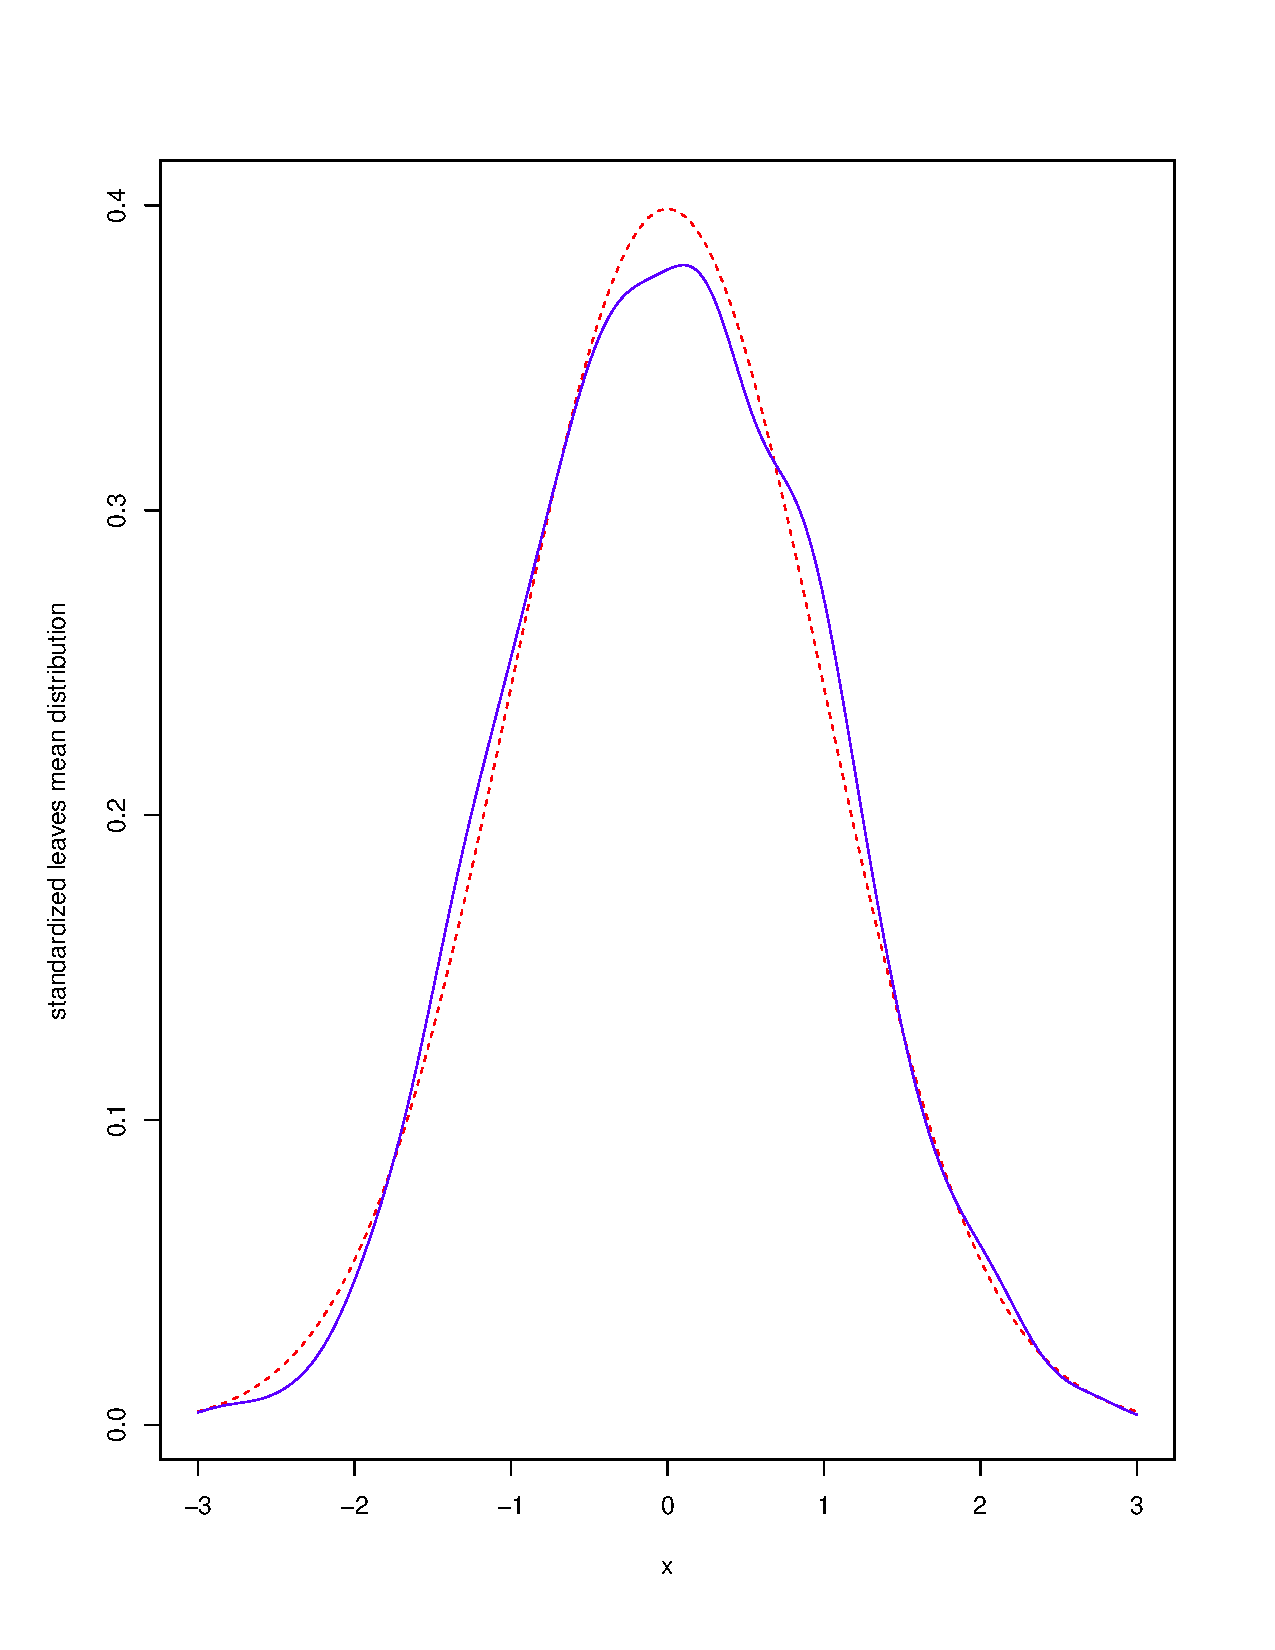
\includegraphics[height=13cm,
  width=13cm]{pictures/repeated-sampling-leaves-mean.pdf}
  \caption{Standardized leaves mean distribution}
  \label{fig:leaves-mean-distribution}
\end{figure}

In \autoref{fig:height-mean-distribution} we report the standardized
mean of leaves.
\begin{figure}[htb]
  \centering
  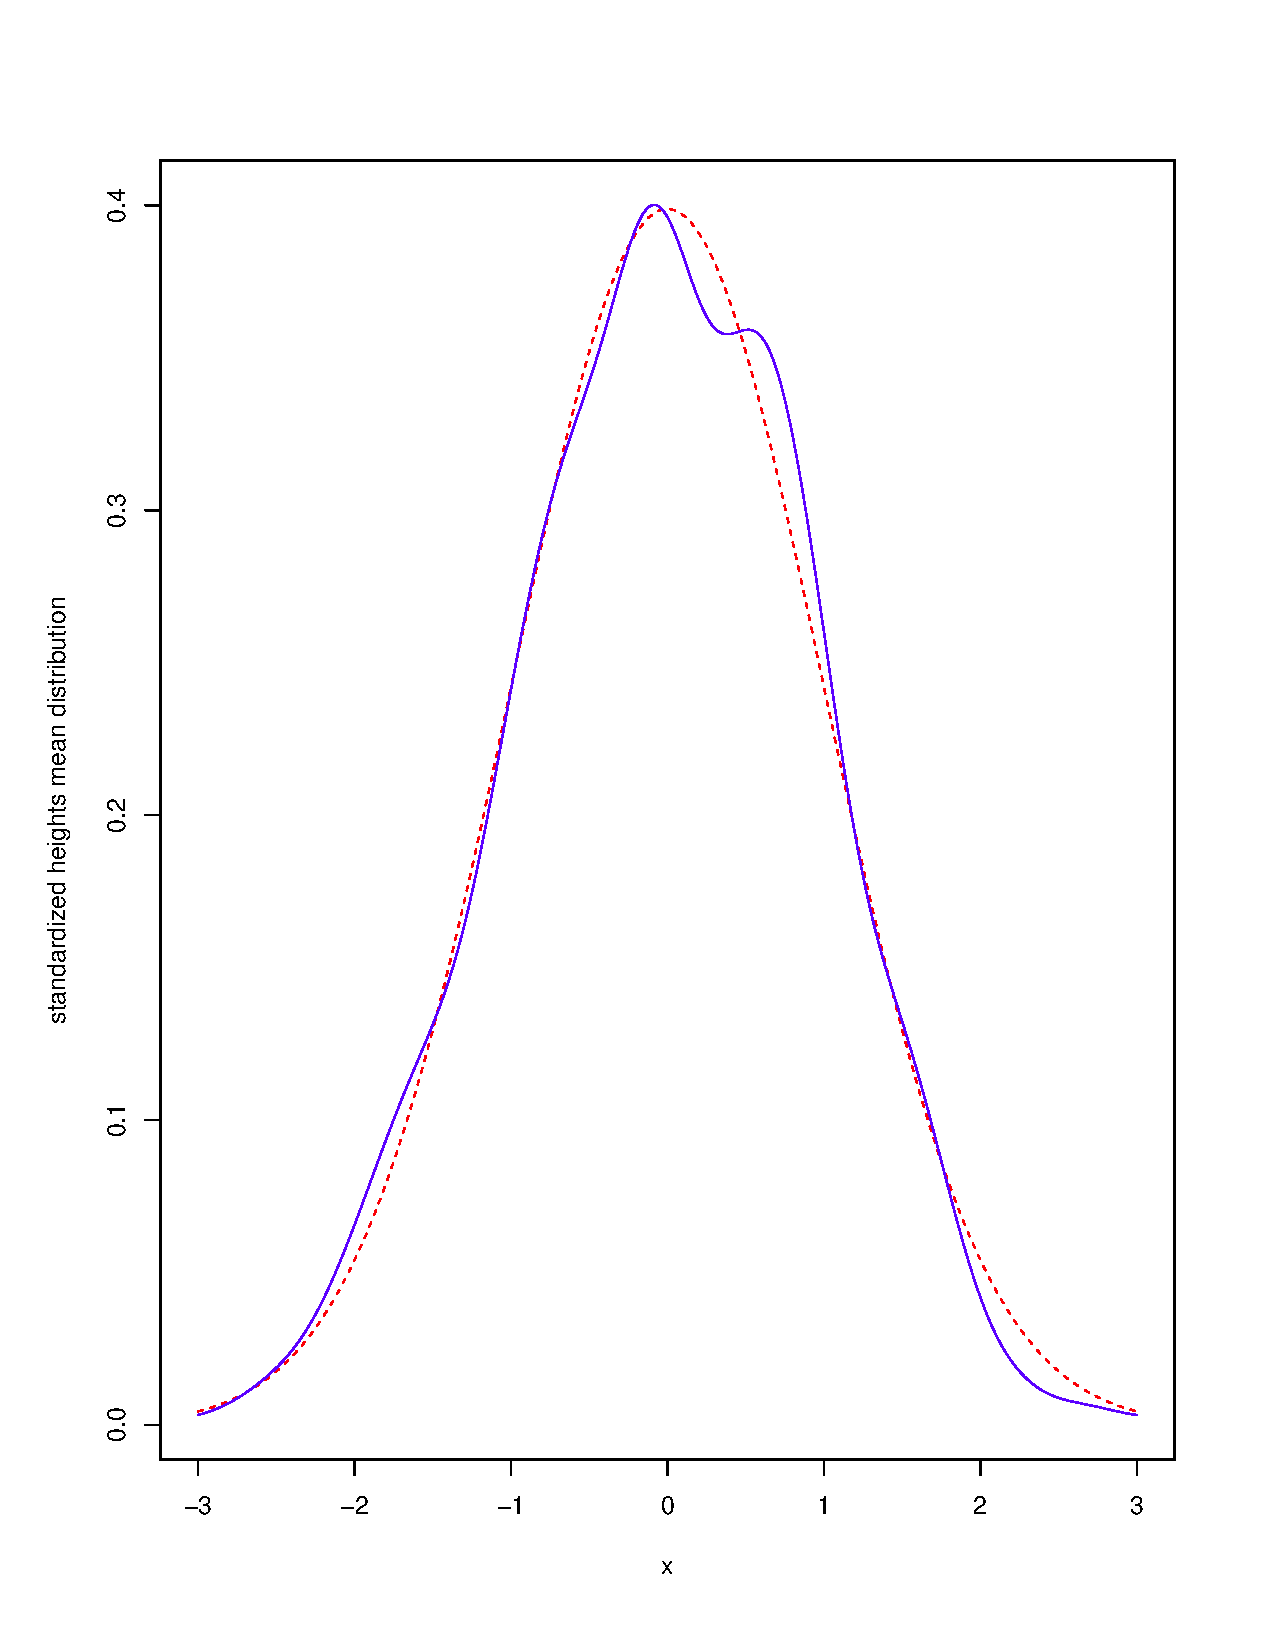
\includegraphics[height=13cm,
  width=13cm]{pictures/repeated-sampling-height-mean.pdf}
  \caption{Standardized height mean distribution}
  \label{fig:height-mean-distribution}
\end{figure}

\section{Drawing trees}

Just for fun, our implementation draw all different trees with $n$
nodes (this implementation is done in OCaml). In
\autoref{fig:binary-trees-with-four-nodes} we report the image with
all binary trees with $4$ nodes.
\begin{figure}[htb]
  \centering
  \rotatebox{90}{
    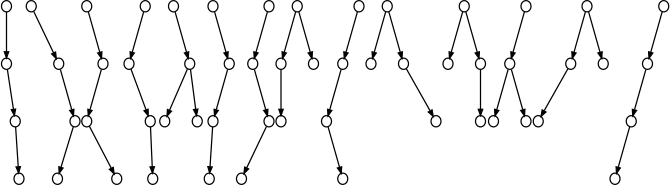
\includegraphics{pictures/binary-trees-with-four-nodes.png}
  }
  \caption{Binary trees with four nodes}
  \label{fig:binary-trees-with-four-nodes}
\end{figure}

\subsection{From bracket representations to binary trees}

In this section we report the algorithm used to build the OCaml tree
objects from bracket representations. The algorithm is recursive:
given an input bracket representation, the algorithm breaks the
representation in smaller representations, which are valid bracket
representations themselves, recurs on each of them and then collects
the results to returns the final answer. In order to describe it more
precisely we distinguish two cases, let $d$ be a bracket
representation:
\begin{itemize}
\item the base of the recursion is for $d=\epsilon$, the empty bracket
  representation. In this case the tree for $d$ is an empty binary
  tree;
\item $d$ cannot be broken into two shorter bracket
  representations. It follows that, since $d$ is however a valid
  bracket representation (ie. $d$ is balanced as we've defined in
  previous sections), it must have the form $d = (M)$, where $M$ is a
  shorter bracket representation (can be the case of $M = \epsilon$
  empty, this is necessary to reach the base of recursion). In this
  case we recur on $M$ combining the result using the following
  strategy:
  \begin{quote}
    let $m$ be the tree corresponding to bracket representation $M$:
    build an empty tree $t$ for bracket representation $d$ attaching
    the root of tree $m$ to the \emph{right} leaf of tree $t$.
  \end{quote}
  For instance assume $d = (())$, hence $M=()$, so we build the
  following tree $t$ for bracket representation $d$:
\begin{verbatim}
       t
      / \
     /   m
    /   / \
\end{verbatim}
\item $d$ can be broken into two shorter bracket representations, that
  is $d = d_1d_2$. Using the toy $d=()(())$ we've $d_1=()$ and
  $d_2=(())$. In this case we recur on both $d_1,d_2$ combining the
  results using the following strategy:
  \begin{quote}
    let $w$ be the tree corresponding to bracket representation $d_1$
    and let $r$ be the tree corresponding to bracket representation
    $d_2$: build a tree $t$ for bracket representation $d$ attaching
    the root of tree $t_1$ to the \emph{left-most} leaf of tree $t_2$.
  \end{quote}
  For example let $d=()(())$ we get the following trees by recursive
  application on $d_1=(),d_2 =(())$ respectively:
\begin{verbatim}
  w       r          r
 / \     / \        / \
        /   o      /   o
       l   / \    w   / \
                 / \
\end{verbatim}
  We attach the tree rooted at $w$ to the \emph{left-most} leaf $l$ of
  tree rooted at $r$ to get the right-most tree rooted at $t$ for $d$
  in the picture above.

  If a bracket representation $d$ can be broken in more shorter
  bracket representations $d_1,\ldots,d_n$ then we break $d$ using the
  \emph{right-most} breakpoint, that is we recur on $d^{\prime} =
  d_1,\ldots,d_{n-1}$ and $d_n$ and proceed as explained above.
\end{itemize}
